%% Compile with: latexmk -pdf frl_three_results.tex

\documentclass[review,12pt,authoryear]{elsarticle}

\usepackage{amsmath,amssymb}
\usepackage{booktabs}
\usepackage{threeparttable}
\usepackage{graphicx}
\graphicspath{{figures/}}

\newcommand{\pp}{\,pp}
\newcommand{\sym}[1]{\ifmmode^{#1}\else\(^{#1}\)\fi}
\journal{Finance Research Letters}

\begin{document}

\begin{frontmatter}

\title{Who Gains from Generative AI Model Releases?}

\author[sdu]{Zhuo Chen\corref{cor1}}
\ead{zhuochen@sdu.edu.cn}
\author[sdu]{Ruishuang Lu}
\cortext[cor1]{Corresponding author.}
\affiliation[sdu]{organization={Center for Economic Research, Shandong University},
city={Jinan}, country={China}}

\begin{abstract}
Stock-market reactions to generative AI releases concentrate in two
ecosystem positions. We study 124 day-verified releases from 2022 to 2026
using 45 securities in the Nasdaq-100 Technology Sector Index, coded by
their relationships to 25 model developers. Hardware suppliers and rival
model developers earn 3.48 and 3.39 percentage points over twenty trading
days; no other position reaches the 5\% significance level. Both premia
emerge in 2025--2026, and the increase for hardware exceeds that for
competitors by about 5 percentage points. Capability scores carry no
positive average premium. A one-standard-deviation increase in capability
widens the hardware premium by about 2 percentage points. The results show
how model-release reactions vary across ecosystem position, market
development, and model capability.
\end{abstract}

\begin{keyword}
Generative AI \sep Event study \sep Ecosystem position \sep
Model capability \sep Technology stocks
\\ \textit{JEL codes}: G14 \sep G12 \sep O33
\end{keyword}

\end{frontmatter}

\section{Introduction}

A generative AI model release reaches several markets at once. It introduces
a product for its developer, signals the growth of an emerging industry to
rival developers, and can shift expected demand for semiconductors, servers,
and networking equipment. Firms commonly grouped under ``AI exposure''
therefore occupy economically distinct positions around the same
announcement. A release can validate the commercial prospects of the model
industry, raising the value of competing developers. It can also change
expectations about demand for the physical inputs used to train and serve
models, raising the value of hardware suppliers.

We measure these position-specific reactions using 124 model releases from
2022 to 2026 and 45 securities in the Nasdaq-100 Technology Sector Index
(NDXT). Release dates are verified against first-party sources. Two coders
independently classify each firm--developer pair into eight ecosystem
positions. The outcome is the firm's cumulative abnormal return over the
twenty trading days following a release.

Release returns concentrate in hardware suppliers and rival model
developers. Hardware suppliers earn 3.48\pp{} and competitors earn
3.39\pp{} relative to firms outside each position. Both coefficients are
significant at 1\% with event-level CR2 inference and at 5\% with
event-and-firm clustering. Cloud platforms, integrators, deployers,
enablers, investors, and listed owners do not reach the 5\% level under
either inference method.

The concentration changes sharply after 2025. Hardware and competitor
coefficients are small and statistically insignificant during 2022--2024,
then rise to 7.18\pp{} and 4.61\pp{} during 2025--2026. The hardware
increase exceeds the competitor increase by 4.86\pp{} under the market
model and 5.03\pp{} under the Fama--French three-factor model. The
difference is significant under event-level and two-way inference.

Model capability further differentiates the hardware response. The
Artificial Analysis intelligence index has no positive pooled return slope.
Its interaction with hardware is positive under both return benchmarks. A
one-standard-deviation increase in capability widens the hardware premium
by approximately 2\pp{}.

The evidence extends asset-pricing work that measures firms' broad exposure
to AI \citep{eisfeldt2023,babina2024}. Position coding separates suppliers,
developers, intermediaries, and users inside the technology sector. The
positive competitor response also connects generative AI releases to the
contagion component of intra-industry news
\citep{lang1992,chen2005}. Taken together, the estimates show two distinct
return profiles within the technology sector: a competitor premium shared
by rival developers and a hardware premium that grows after 2025 and with
model capability. The results document position-level variation in how
technology stocks respond to model releases.

\section{Data and Empirical Design}\label{sec:data}

The event pipeline begins with public model chronologies and benchmark
records. We consolidate same-day releases from the same model family and
verify dates using vendor announcements, release notes, repositories, and
archived first captures. Day-level evidence is available for 125 events.
One identity-inconsistent event is excluded, leaving 124 releases: 3 in
2022, 8 in 2023, 45 in 2024, 59 in 2025, and 9 in 2026. Eighty-seven
language-model events have a comparable Artificial Analysis intelligence
score.

The firm universe contains the 45 securities listed in the NDXT constituent
file dated May 1, 2026. They represent 44 issuers because Alphabet has two
share classes. Two independent coders classify 1,125 firm--developer pairs,
covering 45 securities and 25 model developers. The eight indicators are
hardware supplier, cloud platform, integrator, deployer, downstream enabler,
competitor, investor, and listed owner. Coding is multi-label. Cell-level
agreement is 98.5\%, and all disagreements are adjudicated under a fixed
codebook.

Hardware suppliers earn primary revenue from semiconductors, servers,
networking, storage, and related physical inputs. Cloud platforms rent
computing capacity and host third-party models. Integrators embed foundation
models in their own software, while deployers use AI inside a broader
business. Downstream enablers implement AI systems for clients. Competitors
develop models in the same modality as the released model. Investor and
owner indicators capture financial ties and listed publishers. A firm can
hold several positions around the same release; each regression includes all
eight indicators jointly.

Daily adjusted returns run from January 2021 through April 2026. The market
model uses the S\&P 500 and an estimation window of $[-200,-11]$.
The second benchmark is the Fama--French three-factor model
\citep{fama1993}. The dependent variable is CAR$[0,20]$. Regressions include
log assets, book-to-market, momentum, volatility, and year fixed effects.
The main sample has 5,441 firm-event observations. We estimate
\begin{equation}
 CAR_{ie}=\alpha+\sum_k\beta_k Position_{iek}
 +\gamma'Z_{ie}+\lambda_y+\varepsilon_{ie}.
\end{equation}
The time specification adds each position's interaction with an indicator
for releases in 2025--2026. The capability specification centers the
intelligence index and interacts it with the hardware indicator. Tables
report exact $p$-values from event-level CR2 and event-and-firm two-way
clustering; stars use event-level CR2 inference \citep{cameron2011}.

The coefficients compare firms holding a given position with the remaining
technology firms around the same set of releases, conditional on the other
positions and firm characteristics. The post-2025 interactions compare that
cross-sectional pricing rule across the two periods. The final contrast
tests whether the change in the hardware coefficient equals the change in
the competitor coefficient.

\section{Results}\label{sec:results}

\subsection{Position-level returns}

Table~\ref{tab:position} shows a sharp cross-sectional concentration.
Hardware and competitor coefficients are similar in magnitude and
statistically indistinguishable. Under the market model, their difference is
0.09\pp{} ($p=0.92$). The other six position coefficients do not reach 5\%
under either inference method.

\begin{table}[t!]
\centering
\begin{threeparttable}
\caption{Ecosystem position and twenty-day abnormal returns}
\label{tab:position}
\scriptsize
\setlength{\tabcolsep}{3.2pt}
\begin{tabular}{lrrrrrr}
\toprule
& \multicolumn{3}{c}{Market model}
& \multicolumn{3}{c}{Three-factor model} \\
\cmidrule(lr){2-4}\cmidrule(lr){5-7}
Position & Coef. & Event $p$ & Two-way $p$
& Coef. & Event $p$ & Two-way $p$ \\
\midrule
Hardware supplier      & 3.476\sym{***} & 0.002 & 0.015 & 3.428\sym{***} & 0.002 & 0.016 \\
Cloud platform         & 1.050 & 0.121 & 0.246 & 1.171\sym{*} & 0.079 & 0.235 \\
Downstream integrator  & 1.315\sym{*} & 0.078 & 0.129 & 1.185 & 0.119 & 0.164 \\
Downstream deployer    & 1.261 & 0.137 & 0.183 & 1.266 & 0.140 & 0.192 \\
Downstream enabler     & 0.251 & 0.802 & 0.781 & $-$0.133 & 0.894 & 0.887 \\
Competitor             & 3.385\sym{***} & $<0.001$ & 0.022 & 3.371\sym{***} & $<0.001$ & 0.037 \\
Investor               & 0.480 & 0.691 & 0.627 & 1.048 & 0.362 & 0.291 \\
Listed owner           & 3.181\sym{*} & 0.070 & 0.113 & 3.229\sym{*} & 0.067 & 0.123 \\
\midrule
Observations           & \multicolumn{3}{c}{5,441}
                       & \multicolumn{3}{c}{5,441} \\
Events                 & \multicolumn{3}{c}{124}
                       & \multicolumn{3}{c}{124} \\
\bottomrule
\end{tabular}
\begin{tablenotes}\footnotesize
\item Notes: Coefficients are percentage points. Regressions include all
eight position indicators, firm controls, and year fixed effects. Event
$p$ uses event-level CR2 inference. Two-way $p$ clusters by event and firm.
Event-CR2 stars: \sym{*} $p<0.10$, \sym{**} $p<0.05$,
\sym{***} $p<0.01$.
\end{tablenotes}
\end{threeparttable}
\end{table}

The hardware coefficient exceeds the average of the four downstream
positions by 2.53\pp{} under the market model and 2.66\pp{} under the
three-factor model. Both contrasts are significant at 1\% under event-level
and two-way inference (Online Appendix Table A3).

The SOXX benchmark sharpens the hardware result. After absorbing broad
semiconductor-sector returns, hardware suppliers earn 2.90\pp{}
($p=0.003$), while competitors earn 3.18\pp{} ($p<0.001$). The hardware
coefficient therefore extends beyond a contemporaneous rise in semiconductor
stocks. The 2.53--2.66\pp{} advantage over downstream firms shows a stronger
release response among hardware suppliers than among downstream firms within
the technology sector.

The competitor coefficient carries a different economic meaning. A rival
developer can lose market share to a new release, yet its value can rise
if the release conveys positive news about the size or adoption of the model
market as a whole. The positive 3.39\pp{} estimate is consistent with this
industry-level channel dominating competitive displacement over the sample
period. Its statistical equality with the hardware estimate makes the time
comparison central to distinguishing the two return profiles.

\subsection{Time variation}

Table~\ref{tab:time} traces the two premia across time. During 2022--2024,
the hardware coefficient is $-1.28$\pp{} and the competitor coefficient is
1.00\pp{} under the market model; both are statistically insignificant.
During 2025--2026, they rise to 7.18\pp{} and 4.61\pp{}, with $p<0.01$
under both inference methods.

\begin{table}[t!]
\centering
\begin{threeparttable}
\caption{Position premia before and after 2025}
\label{tab:time}
\scriptsize
\setlength{\tabcolsep}{1.9pt}
\begin{tabular}{lrrrrrr}
\toprule
& \multicolumn{3}{c}{Market model}
& \multicolumn{3}{c}{Three-factor model} \\
\cmidrule(lr){2-4}\cmidrule(lr){5-7}
Estimate & Coef. & Event $p$ & Two-way $p$
& Coef. & Event $p$ & Two-way $p$ \\
\midrule
Hardware, 2022--2024
 & $-$1.285 & 0.463 & 0.431 & $-$1.710 & 0.317 & 0.316 \\
Competitor, 2022--2024
 & 1.001 & 0.427 & 0.524 & 0.685 & 0.593 & 0.680 \\
Hardware, 2025--2026
 & 7.185\sym{***} & $<0.001$ & $<0.001$ & 7.439\sym{***} & $<0.001$ & $<0.001$ \\
Competitor, 2025--2026
 & 4.607\sym{***} & $<0.001$ & 0.003 & 4.802\sym{***} & $<0.001$ & 0.004 \\
\addlinespace
Post-2025 change, hardware
 & 8.469\sym{***} & $<0.001$ & 0.005 & 9.149\sym{***} & $<0.001$ & 0.004 \\
Post-2025 change, competitor
 & 3.606\sym{**} & 0.018 & 0.064 & 4.116\sym{***} & 0.009 & 0.035 \\
Hardware change minus competitor change
 & 4.863\sym{***} & 0.001 & 0.021 & 5.032\sym{***} & 0.001 & 0.022 \\
\bottomrule
\end{tabular}
\begin{tablenotes}\footnotesize
\item Notes: Coefficients are percentage points from a pooled regression
containing all position indicators and their interactions with a
2025--2026 indicator. Controls and inference follow
Table~\ref{tab:position}.
Event-CR2 stars: \sym{*} $p<0.10$, \sym{**} $p<0.05$,
\sym{***} $p<0.01$.
\end{tablenotes}
\end{threeparttable}
\end{table}

Both positions strengthen after 2025, but the hardware increase is
4.86--5.03\pp{} larger. Hardware therefore has the stronger post-2025
response.

The horizon profile in Figure~\ref{fig:profile} shows how the late-period
premia accumulate. In 2025--2026, hardware and competitor coefficients are
small on the release date and rise over the following twenty trading days.
Hardware reaches 7.7\pp{} in the window-by-window specification, while the
competitor coefficient reaches 5.6\pp{}. The growing distance between the
two lines mirrors the formal difference-in-changes test.

\begin{figure}[htbp]
\centering
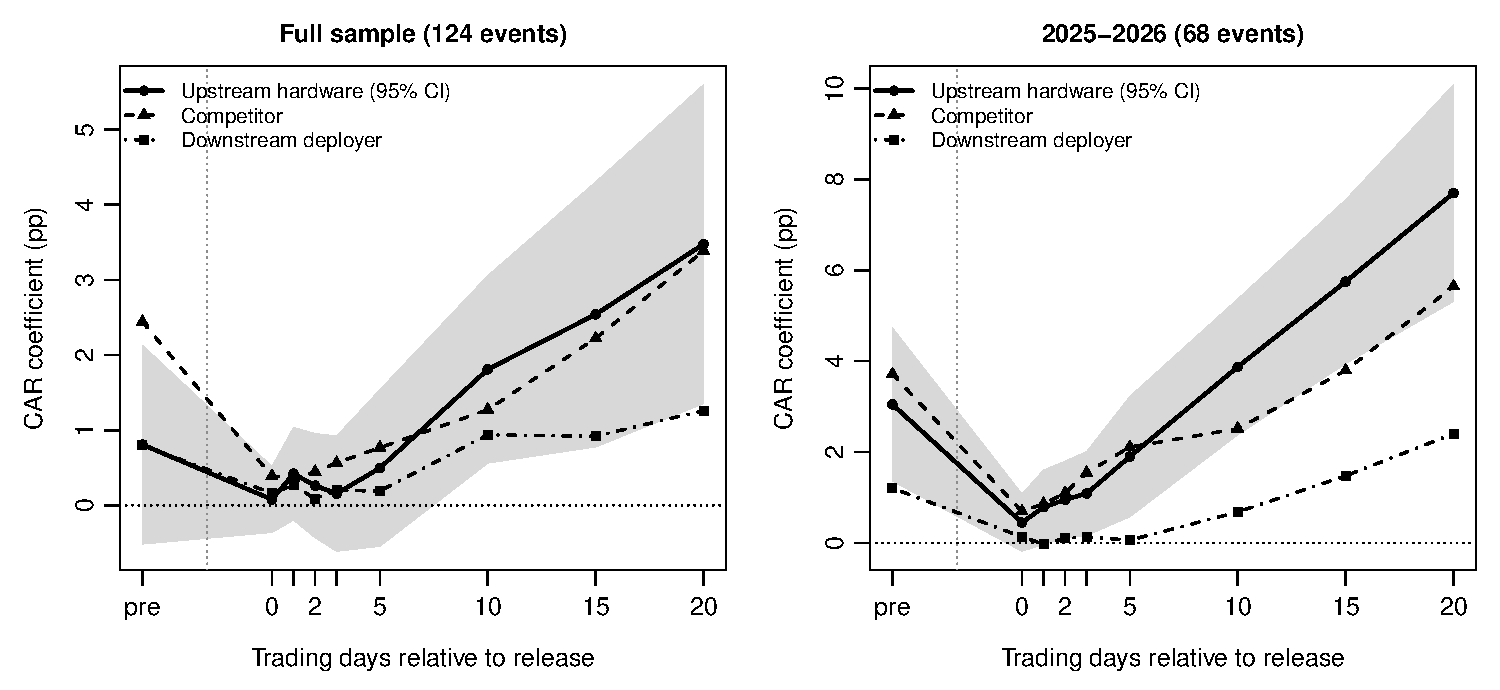
\includegraphics[width=0.92\textwidth]{fig1_car_profile}
\caption{Cumulative abnormal returns by ecosystem position. Coefficients
come from market-model regressions with firm controls and year fixed
effects. The shaded area is the 95\% event-clustered CR2 confidence interval
for hardware. The pre-event point is CAR$[-10,-2]$; the remaining points
cumulate from the release date.}
\label{fig:profile}
\end{figure}

\subsection{Capability and the hardware premium}

The pooled capability slope is $-0.059$\pp{} per index point under the
market model and $-0.080$\pp{} under the three-factor model
(Table~\ref{tab:capability}). Capability therefore carries no positive
average premium.

\begin{table}[t!]
\centering
\begin{threeparttable}
\caption{Model capability and the hardware premium}
\label{tab:capability}
\scriptsize
\setlength{\tabcolsep}{3.2pt}
\begin{tabular}{lrrrrrr}
\toprule
& \multicolumn{3}{c}{Market model}
& \multicolumn{3}{c}{Three-factor model} \\
\cmidrule(lr){2-4}\cmidrule(lr){5-7}
Term & Coef. & Event $p$ & Two-way $p$
& Coef. & Event $p$ & Two-way $p$ \\
\midrule
Capability, pooled
 & $-$0.059\sym{*} & 0.071 & 0.082 & $-$0.080\sym{**} & 0.030 & 0.030 \\
Hardware at mean capability
 & 1.853\sym{**} & 0.046 & 0.068 & 1.950\sym{**} & 0.038 & 0.056 \\
Capability $\times$ hardware
 & 0.154\sym{**} & 0.045 & 0.051 & 0.162\sym{**} & 0.034 & 0.039 \\
\midrule
Observations
 & \multicolumn{3}{c}{3,842} & \multicolumn{3}{c}{3,842} \\
Events
 & \multicolumn{3}{c}{87} & \multicolumn{3}{c}{87} \\
\bottomrule
\end{tabular}
\begin{tablenotes}\footnotesize
\item Notes: Coefficients are percentage points. Capability is the
Artificial Analysis intelligence index. The interaction regressions center
the index before multiplying it by the hardware indicator. All
specifications include firm controls and year fixed effects.
Event-CR2 stars: \sym{*} $p<0.10$, \sym{**} $p<0.05$,
\sym{***} $p<0.01$.
\end{tablenotes}
\end{threeparttable}
\end{table}

The interaction is 0.154\pp{} per index point under the market model and
0.162\pp{} under the three-factor model. The intelligence index has a
standard deviation of 12.7 points, so a one-standard-deviation increase
widens the hardware premium by 1.95--2.06\pp{}. Capability therefore shifts
the cross-sectional allocation of release returns toward hardware suppliers.

The interaction links technical performance to cross-sectional variation
in the hardware premium. A higher benchmark score is associated with a
larger return difference between hardware suppliers and other firms. One
interpretation is stronger expected demand for computing inputs. The same
position also shows the largest post-2025 increase.

\section{Conclusion}\label{sec:conclusion}

Generative AI model releases are priced unevenly across the technology
sector. Hardware suppliers and rival model developers show positive
twenty-day abnormal returns. Both premia emerge after 2025, with an additional
hardware increase of about 5\pp{}. Model capability widens the hardware
premium by about 2\pp{} per standard deviation. Ecosystem position, market
development, and model capability jointly shape the cross-section of
release-related stock returns.

The results highlight the value of distinguishing ecosystem positions when
studying AI-related news. Hardware and competitor premia are similar over
the full period, but their time profiles diverge after 2025, and only the
hardware premium rises with model capability.

\section*{Data availability}

The event pipeline, coding decisions, estimation code, and complete
robustness results are available from the authors. The online appendix
reports the coding protocol, alternative benchmarks, dependence
adjustments, non-overlapping-event samples, and composition tests.

\begin{thebibliography}{00}
\expandafter\ifx\csname natexlab\endcsname\relax\def\natexlab#1{#1}\fi

\bibitem[Babina et al.(2024)]{babina2024}
Babina, T., Fedyk, A., He, A., Hodson, J., 2024. Artificial intelligence,
firm growth, and product innovation. Journal of Financial Economics 151,
103745.

\bibitem[Cameron et al.(2011)]{cameron2011}
Cameron, A.~C., Gelbach, J.~B., Miller, D.~L., 2011. Robust inference
with multiway clustering. Journal of Business \& Economic Statistics 29,
238--249.

\bibitem[Chen et al.(2005)]{chen2005}
Chen, S.-S., Ho, K.~W., Ik, K.~H., 2005. The wealth effect of new product
introductions on industry rivals. Journal of Business 78, 969--996.

\bibitem[Eisfeldt et al.(2023)]{eisfeldt2023}
Eisfeldt, A.~L., Schubert, G., Zhang, M.~B., 2023. Generative AI and firm
values. NBER Working Paper 31222.

\bibitem[Fama and French(1993)]{fama1993}
Fama, E.~F., French, K.~R., 1993. Common risk factors in the returns on
stocks and bonds. Journal of Financial Economics 33, 3--56.

\bibitem[Lang and Stulz(1992)]{lang1992}
Lang, L.~H.~P., Stulz, R.~M., 1992. Contagion and competitive
intra-industry effects of bankruptcy announcements. Journal of Financial
Economics 32, 45--60.

\end{thebibliography}

\end{document}
